\section{Workgroups}

\subsection{Continuous integration}
\definecolor{ornl_green}{RGB}{42, 100, 51}
\definecolor{snl_blue}{RGB}{75, 165, 226}
\definecolor{cea_red}{RGB}{204, 43, 40}
% \definecolor{github_black}{RGB}{255, 255, 255}
\definecolor{hpsf_purple}{RGB}{110, 39, 107}
\definecolor{nersc_blue}{RGB}{14, 43, 80}


\begin{frame}[fragile]{Founding of CI-WG}
  \begin{center}
\textbf{Kokkos founded a working group for continuous integration}
\vspace{1cm}
  \end{center}

    Objectives
    \begin{itemize}
      \item{Redistribute testing to more institutions}
      \item{Increase coverage}
      \item{Diversify knowledge to increase robustnes}
    \end{itemize}

\end{frame}

\begin{frame}[fragile]{CI coverage}

  \begin{center}
    \begin{minipage}{.45\textwidth}
    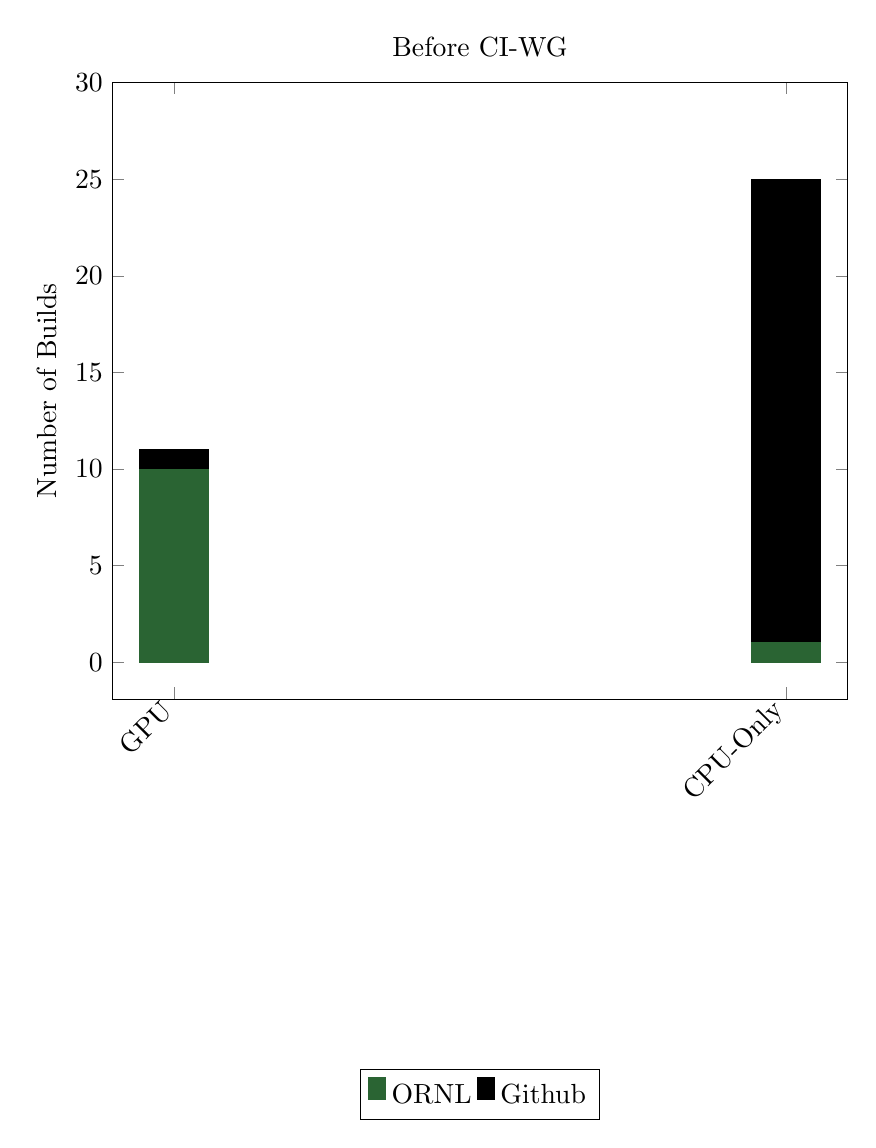
\begin{tikzpicture}
  \begin{axis}[
    title={Before CI-WG},
    ybar stacked,
    ymax=30,
    bar width=25pt,
    symbolic x coords={GPU, CPU-Only},
    xticklabel style={rotate=45,anchor=east},
    xtick=data,
    width=0.9\textwidth,
    legend style={at={(0.5,-0.60)},
      anchor=north,legend columns=-1},
    ylabel=Number of Builds]
  \addplot+[ybar,color=ornl_green] plot coordinates {(GPU,10) (CPU-Only,1)};
  \addplot+[ybar,color=black] plot coordinates {(GPU,1) (CPU-Only,24)};
  \legend{\strut ORNL, \strut Github}
  % \legend{\strut ORNL, \strut SNL, \strut CEA, \strut Github, \strut HPSF, \strut NERSC}
  \end{axis}
\end{tikzpicture}
\end{minipage}
\begin{minipage}{.45\textwidth}
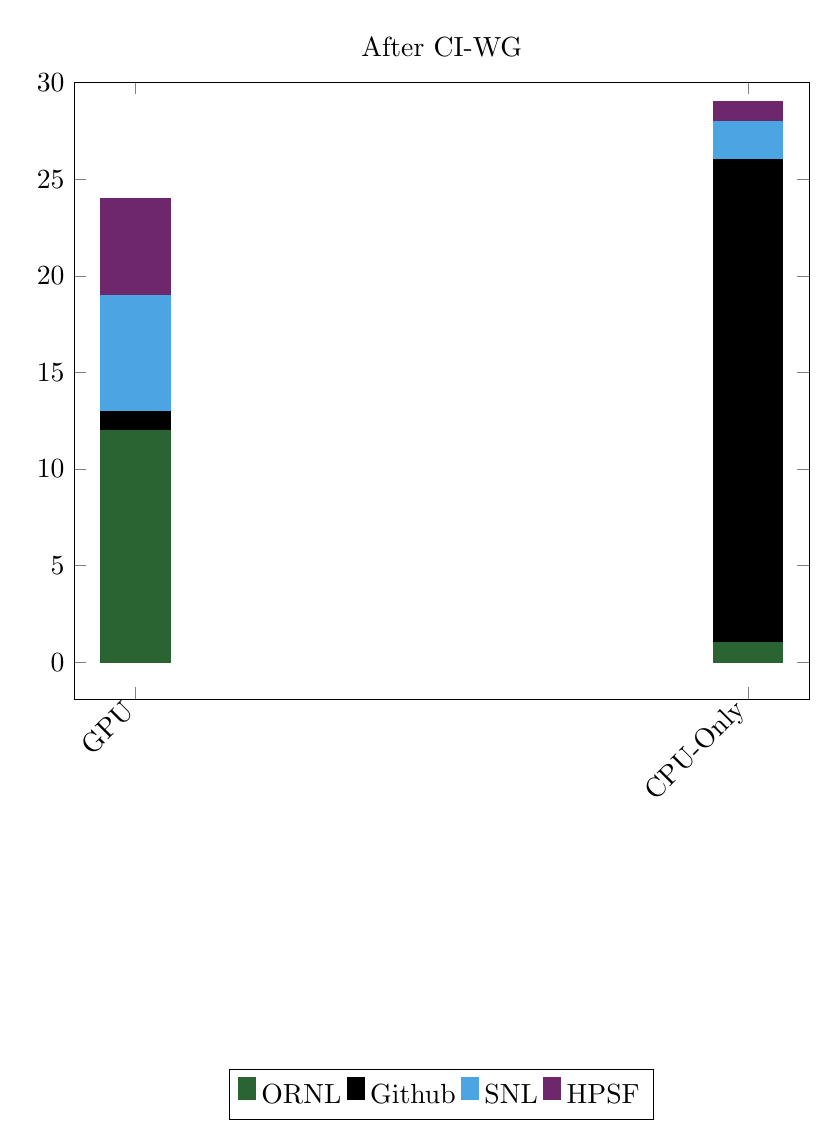
\begin{tikzpicture}
  \begin{axis}[
    title={After CI-WG},
    ybar stacked,
    ymax=30,
    bar width=25pt,
    symbolic x coords={GPU, CPU-Only},
    xticklabel style={rotate=45,anchor=east},
    xtick=data,
    width=0.9\textwidth,
    legend style={at={(0.5,-0.60)},
      anchor=north,legend columns=-1}]
  \addplot+[ybar,color=ornl_green] plot coordinates {(GPU,12) (CPU-Only,1)};
  \addplot+[ybar,color=black] plot coordinates {(GPU,1) (CPU-Only,25)};
  \addplot+[ybar,color=snl_blue] plot coordinates {(GPU,6) (CPU-Only,2)};
  \addplot+[ybar,color=hpsf_purple] plot coordinates {(GPU,5) (CPU-Only,1)};
  \legend{\strut ORNL, \strut Github, \strut SNL, \strut HPSF}
  \end{axis}
\end{tikzpicture}
\end{minipage}
  \end{center}

\end{frame}

\begin{frame}[fragile]{Nightlies coverage}

  \begin{center}
    \begin{minipage}{.45\textwidth}
    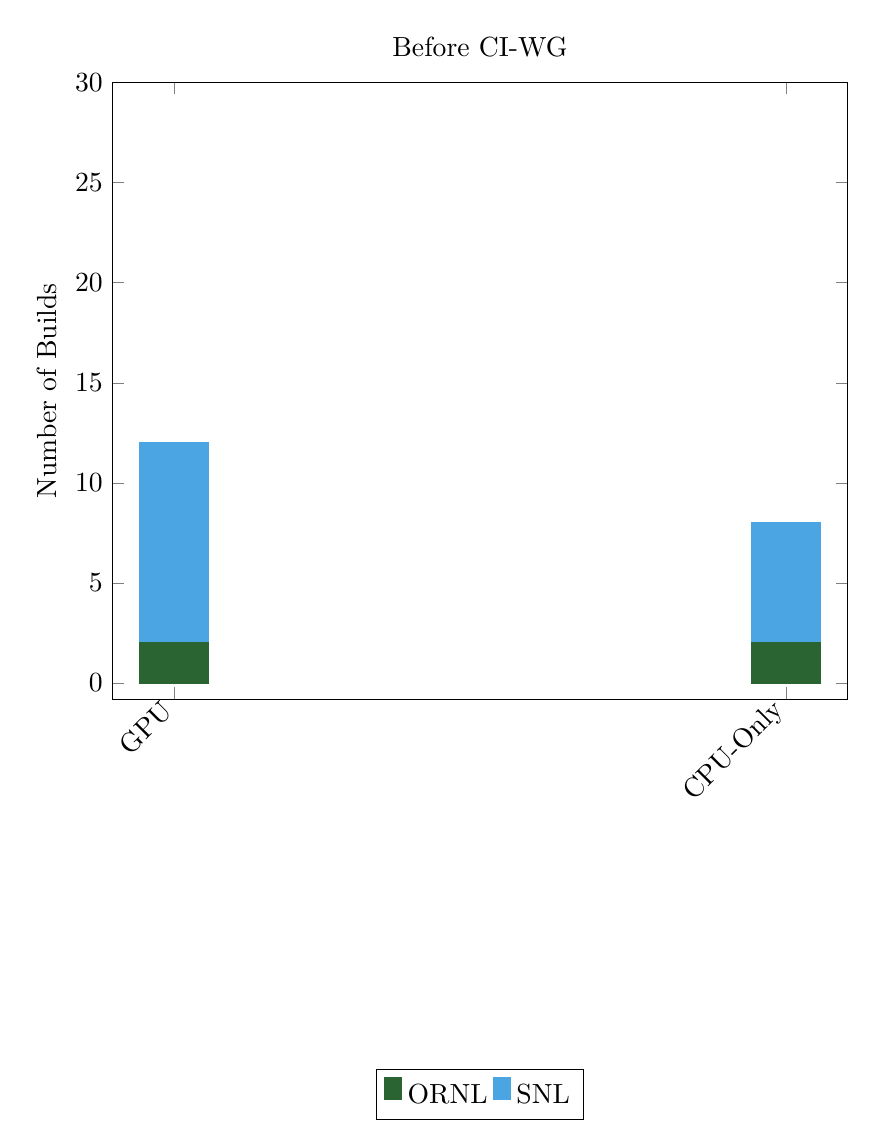
\begin{tikzpicture}
  \begin{axis}[
    title={Before CI-WG},
    ybar stacked,
    ymax=30,
    bar width=25pt,
    symbolic x coords={GPU, CPU-Only},
    xticklabel style={rotate=45,anchor=east},
    xtick=data,
    width=0.9\textwidth,
    legend style={at={(0.5,-0.60)},
      anchor=north,legend columns=-1},
    ylabel=Number of Builds]
  \addplot+[ybar,color=ornl_green] plot coordinates {(GPU,2) (CPU-Only,2)};
  \addplot+[ybar,color=snl_blue] plot coordinates {(GPU,10) (CPU-Only,6)};
  \legend{\strut ORNL, \strut SNL}
  \end{axis}
\end{tikzpicture}
\end{minipage}
\begin{minipage}{.45\textwidth}
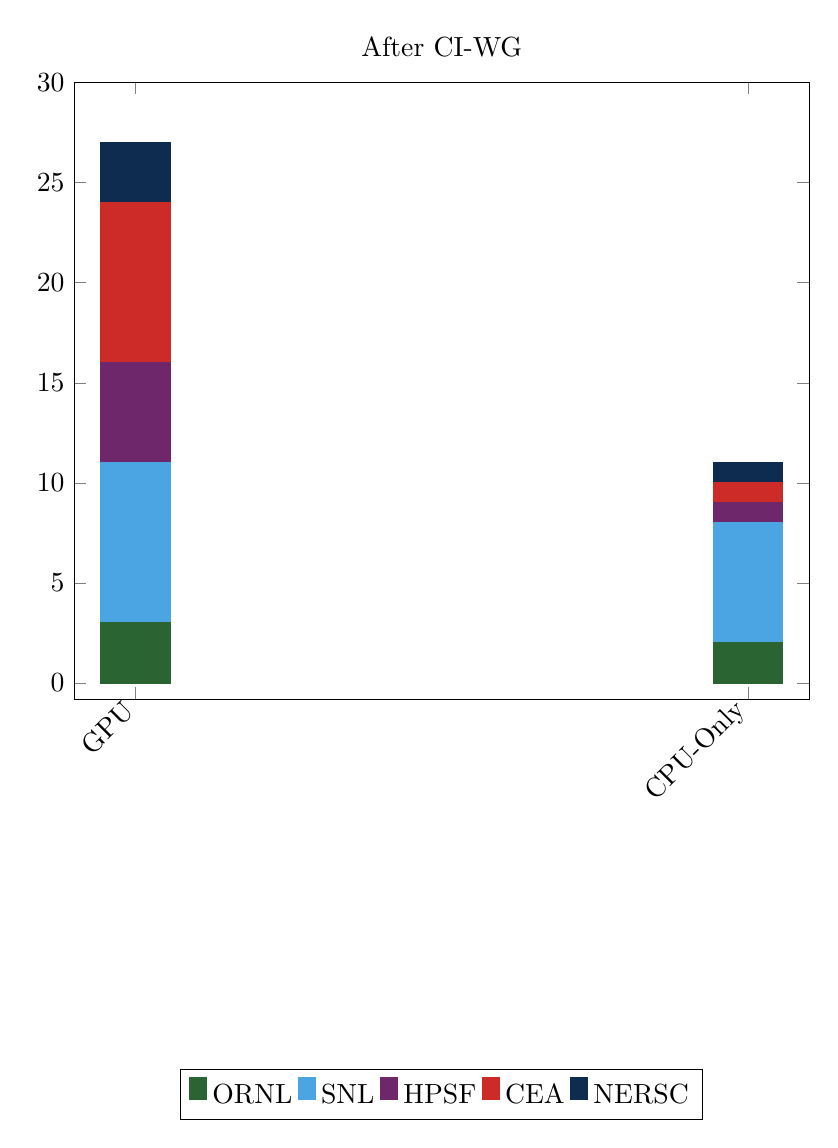
\begin{tikzpicture}
  \begin{axis}[
    title={After CI-WG},
    ybar stacked,
    ymax=30,
    bar width=25pt,
    symbolic x coords={GPU, CPU-Only},
    xticklabel style={rotate=45,anchor=east},
    xtick=data,
    width=0.9\textwidth,
    legend style={at={(0.5,-0.60)},
      anchor=north,legend columns=-1}]
  \addplot+[ybar,color=ornl_green] plot coordinates {(GPU,3) (CPU-Only,2)};
  \addplot+[ybar,color=snl_blue] plot coordinates {(GPU,8) (CPU-Only,6)};
  \addplot+[ybar,color=hpsf_purple] plot coordinates {(GPU,5) (CPU-Only,1)};
  \addplot+[ybar,color=cea_red] plot coordinates {(GPU,8) (CPU-Only,1)};
  \addplot+[ybar,color=nersc_blue] plot coordinates {(GPU,3) (CPU-Only,1)};
    \legend{\strut ORNL, \strut SNL, \strut HPSF, \strut CEA, \strut NERSC}
  \end{axis}
\end{tikzpicture}
\end{minipage}
  \end{center}

\end{frame}

\subsection{Build and packaging}
\begin{frame}[fragile]{Build and packaging}
    \begin{center}
        \begin{itemize}
            \item \textbf{Mission}: To streamline the process of building and distributing the Kokkos performance portability libraries. Our focus is on developing and maintaining robust build systems, creating consistent and user-friendly packaging solutions, and ensuring compatibility across various platforms and environments.
            \item \textbf{Achievements}: Created a space for discussing spack packaging of Kokkos.
            \item \textbf{Roadmap}: Maintain Kokkos integration in package managers. Investigate if Godbolt can host Kokkos with CUDA backend. Add container support for tutorials.
        \end{itemize}
    \end{center}
\end{frame}